% Chapter 2

\chapter{State of Art}
\label{chap:Chapter2}

This chapter intends to present some essential knowledge about the most relevant topics, namely Portuguese Sign Language, Information Retrieval, Information Extraction, Text Mining.
It also presents a description of the readability metrics, work related to this solution and technologies that are mentioned through out this report.

\section{Língua Gestual Portuguesa}

Sign language was created to allow people to communicate through signs instead of sounds.
This is particularly useful for those that have some hearing impairment that made them incapable of learning to communicate through sounds.

The \gls{LGP} has its origins in the first Portuguese school for the deaf that was created in Lisbon by a Swedish educator by the name Pär Aron Borg.
This educator introduced an adaptation of the Swedish manual alphabet that was used by the deaf community to communicate.
Even though, currently, there are no similarities in the vocabulary of the \gls{LGP} and the Swedish sign language, the alphabet still shows the common origin\cite{oliveira2013tradutor}\cite{escudeiro2015virtual}

According to the Portuguese Deaf Association there are around 150000 people with some type of hearing impairment and around 30000 of those that use the \gls{LGP}\cite{gaspar2015if2lgp}.
This language was approved by the Constitution of the Portuguese Republic, in 1997, and became one of the three official languages in Portugal.

In the context of a sign language, a sign, is used to represent an idea and it is composed by the movement and position of the upper limbs.
Paula Escudeiro et al.\cite{escudeiro2015virtual} present the components of a \gls{LGP} sign as manual and non-manual.

The manual component consists in every variables related to hands which includes:
\begin{itemize}
    \item \textbf{Configuration of the hand} - The form that each hand takes while executing a gesture.
    \item \textbf{Orientation of the palm of the hand} - Some configurations only differ in the palm's orientation.
    \item \textbf{Location of articulation} - The area where the gesture is performed (Connected to a body part, touching a body part or just in front of the user).
    \item \textbf{Movement of the hand} - The motion of the hands during the execution of a gesture.
\end{itemize}

The non-manual component consists in the other variables that take part when representing a sign, which includes:
\begin{itemize}
    \item \textbf{Body movement} - The leaning of the torso which represents a temporal context.
    \item \textbf{Facial expressions} - Used to add a sense of emotion to the speech.
\end{itemize}

There are three ways to structure a sentence In \gls{LGP}: SOV (subject-object-verb), SVO (subject-verb-object) or OSV (object-subject-verb).
The predominate sequence used is the SOV\cite{sousa2012interpretaccao}\cite{correia2015linguas} but it's entirely up to the user to chose the structure to use.
Since there are no rule for this, the same user may choose to use a different structure for different sentences\cite{martins2011letra}.
The other parts used to construct a sentence in Portuguese, like the propositions and the articles, are omitted when converted to \gls{LGP}\cite{bento2014avatares}.

Some grammatical characteristics of the Portuguese Sign Language are\cite{bento2014avatares}:
\begin{itemize}
    \item In most cases the prefix "women" is used to identify the female version of a being while the male version is identified by the lack of a prefix "male".
    \item To describe a quantity of a given subject a number can be added or the use of the suffix "many".
    \item To represent temporal placement its used the suffix "past" or "future" to the verb.
    \item The negation of a sentence is defined by the word "not" at the end.
    \item It is used an interrogative pronoun at the end of the sentence to represent it as a question.
\end{itemize}

As already mentioned in the Introduction the \gls{LGP} lexicon is quite small in comparison to Portuguese.
So many Portuguese words are represented by a logical decomposition of its meaning.
Using the word "Laranjeira" as an example, this the Portuguese word for orange tree.
Since there are no sign for this word, it is represented by the signs "Árvore" and "Laranja" (Tree and Orange respectively).

However when a \gls{LGP} user is faced with a word that he does not know its meaning he will spell each letter of the word.
For short words this can be a practical solution but for long words like "Nanotecnologia" not so much.
Spelling this word would require 13 sings while representing its meaning would take around 7 signs (e.g. Ciência, Estudar, Manipular, Materia, Tamanho, Muito and Pequeno).

\section{Information Retrieval}

The search for information is a human activity that was always present.
The World Wide Web brought the commodity of searching information from within one's home, where before it was required to go to a place that stored said information, mainly libraries.

Information Retrieval (IR), as the name suggests, is the act of retrieving information from a source, but this definition can be very broad.
Manning et al.\cite{manning2008introduction} wrote on their book that Information Retrieval is finding materials of an unstructured nature that satisfies an information need from within large collections.

In Figure \ref{fig:iret} is shown a visual representation of the main functionality of Information Retrieval: getting a set of relevant documents.
\begin{figure}[H]
\centering
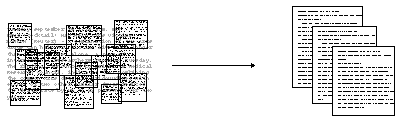
\includegraphics[scale=0.65]{ch2/assets/retrieve.png}
    \caption[InformationRetrival]{Visual representation of Information Retrieval\footnote{Image source: https://gate.ac.uk/ie/}}
\label{fig:iret}
\end{figure}

The best, and most used, example of the application of Information Retrieval is a web search engine such as Google\footnote{https://www.google.com/}.
When a search is performed in this engine, an algorithm will compare the text of the query with the text of a page and decide whether the page contains the information that is being sought.
At its core, Information Retrieval aims to understand and model how people compare texts in order to design algorithms to accurately perform this comparison\cite{croft2010search}.

\section{Information Extraction}

As society became more data oriented having access to both structured and unstructured data became easy.
The difference between those those types of data is that structured data is semantically defined for a target domain and is interpreted with respect to category and context.
Therefor the need for applications capable of extracting structured data had increased.

Information Extraction (IE) is the name given to the process of automatically extracting structured information from an unstructured sources, mainly texts.

In Figure \ref{fig:iext} is shown a visual representation of the main functionality of Information Extraction: getting facts out of documents.
\begin{figure}[H]
\centering
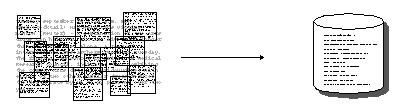
\includegraphics[scale=0.65]{ch2/assets/extract.png}
    \caption[InformationExtraction]{Visual representation of Information Extraction\footnote{Image source: https://gate.ac.uk/ie/}}
\label{fig:iext}
\end{figure}

The result of an IE process is different for every case since it can be tailored according to the application needs.
Nowadays this applications can be used to fulfill personal, scientific and enterprise needs.

With the evolution of technology, IE also evolved and different techniques for the extraction of information were developed.
This techniques are the following: Rule-based, Statistical, Hybrids (both rule-based and statistical) and Conditional Random Fields\cite{sarawagi2008information}.

A rule-based approach was used by Del Gaudio et al.\cite{del2007automatic}.
In this paper the authors created a IE system that was capable extracting the definition of a Portuguese words from texts written in Portuguese.

A statistical approach was used by Ventura\cite{ventura2014automatic}.
In his PhD report, he presented an alternative approach to the extraction of relevant terms from text.
Since relevance of a term is not conceptual, the author proposes to extract all concepts, which have a less fuzzy nature, and let the downstream application decide the relevance of those concepts.
A concept in the text mining area consists of a word or sequence of words which possess semantic value.

A conditional random fields approach was used by Kaijian Liu\cite{liu2017ontology}.
This this paper, the authors proposed this approach to extract information that described existing deficiencies and performed maintenance actions from bridge inspection reports.

\section{Text Mining}

Text mining stands in between the fields of Data Mining, Information Retrieval, Information Extraction, Machine Learning, Knowledge Discovery and Natural Language Processing since its described as the process to find implicit, previously unknown, and potentially useful information from a large data source, which in this case is text.

Information Extraction is the field most similar to Text Mining.
Their main difference is that Information Extraction involves the extraction of specific structured information and predefined relations while Text Mining focus on discovering general unsuspected information and new relations\cite{mulins2008information}.

The goal of text mining is to combines a human's linguistic capabilities with the processing power of a computer\cite{fan2006tapping}.
To accomplish this it borrows many algorithms and techniques from the surrounding fields.

Some of the most used Text Mining techniques\cite{gupta2009survey}\cite{tseng2007text}\cite{patel2012text} are the following:
\begin{itemize}
    \item \textbf{Summarization} - This technique consists in condensing the source text into a shorter version by reducing its detail while retaining the main points and overall meaning.
            Text summarization methods can belong into two categories: extractive and abstractive.
            The extractive methods focus in selecting important sentences or paragraphs and concatenating them into a shorter form.
            This importance is based on statistical and linguistic features of each sentences.
            The abstractive methods attempt to create a human-like interpretation of the document, and express those concepts in natural language.
            Linguistic methods are used to create this interpretation and the new shorter text that contains the most important information from the original text.
        \item \textbf{Categorization} - This technique involves identifying the main theme of a document by placing the document in a predefined category.
            To accomplish this a computer program will count the occurrence of each word that appear.
            This value will be used to identify the main topics covered by the document.
            Tools that use Categorization normally have a method for ranking the documents by the quantity of content in a particular topic.
        \item \textbf{Clustering} - This technique seeks to identify and organize similar documents into relevant subgroups or clusters.
            The main difference to Categorization is that this groups are defined during the execution instead of predefined.
            Another benefit of this technique is that a document can belong to multiple clusters.
        \item \textbf{Concept linkage} - This technique connects related documents by identifying their shared concepts.
            The primary goal of Concept Linkage is to provide browsing for information instead of searching for it as in Information Retrieval.
        \item \textbf{Question Answering} - This technique uses natural language queries, which goal is to find the best answer to a given question.
            A website that is capable of performing Question Answering, can allow a user to "ask" questions to the computer to get and exact or related answer.
        \item \textbf{Information Visualization} - This technique, in addition to simple searching, allows the browsing of text sources in a visual hierarchy or map.
            There are three steps required for visualization: Data preparation, Data analysis and Extraction and Visualization mapping.
            Information visualization can be used to narrow down a broad range of documents and explore related topics.
\end{itemize}

\section{Online Dictionaries}

Dictionaries in the most common form are books, that list the words of a language in alphabetic order followed by their meaning.
Whit the evolution of technology, this dictionaries also evolved into an online version that is more practical and easily accessible.

One of the most known online dictionaries with \gls{LGP} content is the Spreadthesign\footnote{https://www.spreadthesign.com/}.
In this dictionary an user can search for a word and if there's a previously recorded video translation for that word, at the site database, it will be displayed for the user.
The search results only display the video of a person performing the corresponding sign, and the possibility to look at the same word in another sign language.

Another online dictionary that provides content for the \gls{LGP} users is the Infopédia\footnote{https://www.infopedia.pt/dicionarios/lingua-gestual}.
Although this is a Portuguese dictionary, it also contains a section for searching words in \gls{LGP}.
Here, the search results, not only provide a video translation of the word, but also an explanation in Portuguese on how to reproduce the sign shown in the video.

Online dictionaries as a solution, is limited by the database of prerecorded videos, and the \gls{LGP} lexicon.
The latter is a problem, because they focus on a direct translation, word to sign, instead of trying to translate the meaning of the word.

\section{Sign Language Interpreter}

Sign language interpreters are people who help bridging the gap between the hearing impaired or deaf individuals and a spoken language.
This can occur in a one-on-one situation as well as in a group setting.

In regard to the sign language interpreters in Portugal, there is CTILG\footnote{http://www.ctilg.pt/}, a company that provides professional \gls{LGP} translation services in workshops, classes, congresses, events and more.
This company is responsible for the live translation of some morning TV shows.

A more affordable solution for a regular \gls{LGP} user, is the Serviin\footnote{http://www.portaldocidadaosurdo.pt/Serviin} which is a service that provides an interpreter to work as a middle-man between a deaf person and a targeted service/company.
This solution is available as a mobile app, with a very low cost for the deaf user, or through a  web app that is free.

This solution is limited by the interpreters own knowledge and their cost.
Also by utilizing this solution, the \gls{LGP} user is sacrificing some of his autonomy.

\section{Readability Metrics}

Readability is the trait that makes text clearer and more accessible to its readers.
The readability metrics are used to calculate a score\cite{meyer2003text}, that relates to the level of education a reader will need, to fully understand the context of a given text.

The existing readability metrics\cite{correia2020evaluation} for the English language are the following:
\begin{itemize}
    \item \textbf{Flesch Reading Ease Score} - This metric outputs a score that ranges from 0 to 100 and the readability levels are mapped to this scores (e.g. 0--30 Very difficult, 31--50 Difficult, etc.).
        Higher values indicate better legibility, intelligibility and readability.
        The initial aim of this metric was to assess the legibility in educational texts.
        To obtain its score this metric takes in consideration: total number of words, total number of sentences and total number of syllables.
    \item \textbf{Flesch-Kincaid Grade Level} - This metric is the recalculation of the Flesch Reading Ease Score.
        Instead of having mapped values, the results are equivalent to the grade level of education required to understand the text (e.g. 8 corresponds to at least the eight grade of education).
    \item \textbf{Gunning Fog Index} - The scores calculated by this metric range from 0 to 20.
        They correspond to the education grade that the reader should have in order to understand the text on the first reading.
        The difference to the FLesch-Kincaid Grade Level is that it takes in consideration the existence of complex words in the text.
        Complex words are words with three or more syllables with some exceptions.
    \item \textbf{Automated Readability Index} - This metric also outputs a score that corresponds to the education grade level of the reader.
        The difference is that it takes in consideration the word length, that is calculated bases on number of characters instead of number of syllables.
    \item \textbf{Coleman-Liau Index} - This metric produces a score that aims to be an approximation of the minimum U.S. education grade level to comprehend a certain text.
        Like the previous metric Automated Readability Index, this too uses the number of characters to calculate the word length.
        The difference is that it only takes in consideration a sample of 100 words.
    \item \textbf{Dale-Chall and New Dale-Chall} - The creators of this formula, took inspiration in the Flesch Reading Ease to calculate a score that relates to the grade level required to comprehend a certain text.
        What makes this metric different from the others is that it takes in consideration the number of "hard" words.
        A word is considered "hard" if it does not appear in a predefined list of familiar and easy to read words for the English language.
        Having words defined in a list allows to adjust the difficulty for different contexts.
    \item \textbf{Simple Measure of Gobbledygook (SMOG)} - This metric also related the resulting score to the grade level.
        What makes this metric unique is that it only takes in consideration the number of polysyllable words in a text.
        Polysyllable words are words with 3 or more syllables and are calculated from a sample of 30 lines (first 10, middle 10 and last 10).
    \item \textbf{Fry Graph} - This metric estimates the required grade level of the reader based on a graph created by the author.
        The graph was built assuming that texts that contained shorter sentences and words with less syllables become more readable.
        To obtain its score, this metric takes in consideration the number of sentences and number of syllables in a sample of 100 words
    \item \textbf{Raygor Estimate Graph} - This metric like the previous Fry Graph, estimates the required grade using a graph.
        The difference is takes in consideration the number of words with six or more characters.
    \item \textbf{FORCAST} - This metric can be used to either indicate the grade level required or the age required.
        Unlike the other metrics, this one is typically used to evaluate multiple-choice quizzes and forms rather than text.
    \item \textbf{SPACHE} - This metric, like the Dale-Chall, is used to calculate the grade level taking in consideration sentence length and the number of unfamiliar words.
        The difference is that its target to determine the readability for third-grade level texts or below.
\end{itemize}

\subsection{Portuguese Readability Metrics}

In 2019, Antunes et al.\cite{antunes2019analyzing} published an article that adapted the values of the metrics used to calculate the readability of text in English so it could be applied to Portuguese.
The adapted readability metrics are presented in Table \ref{table:ptformulas}.

\begin{table}[H]
    \centering
    \caption{Adjusted Portuguese formulas.}
    \label{table:ptformulas}
    \begin{tabular}{l|l}
        \hline
        {} & {\bfseries Formula} \\
        \hline
        SMOG & \(16.830 \times \sqrt{CW \times 30 \div SE} - 23.809\)  \\
        \hline
        Flesch-Kincaid & \(0.883 \times WO \div SE + 17.347 \times SY \div WO - 41.239\) \\
        \hline
        ARI & \(6.286 \times CH \div WO + 0.927 \times WO \div SE - 36.551\) \\
        \hline
        Coleman Liau & \(5.730 \times CH \div WO - 171.365 \times SE \div WO - 6.662\) \\
        \hline
        Gunning Fog & \(0.760 \times WO \div SE + 58.600 \times CW \div WO - 12.166\) \\
        \hline
        \multicolumn{2}{l}{CH - characters, CW - complex words, SY - syllables, WO - words, SE - sentences}
    \end{tabular}
\end{table}

\section{Related Work}

After extensive research, this project seems to be the first to try to accomplish the goal of generating a definition to a given word or expression using Text Mining, Information Retrieval and Information Extraction.

Trying to achieve a similar goal using a different approach, Noraset Thanapon et al.\cite{noraset2016definition} chose a Deep Learning approach, that used a \gls{RNN} model that used distributed representations of words, also known as word embeddings, to generate dictionary representations.
The models were trained using a pre-defined data set.

Ni Ke et al.\cite{ni2017learning} also chose a Deep Learning approach and a \gls{RNN} model to generate a explanation of a given word or expression from "tweets" which is the name given to the posts made by the users of Twitter\footnote{https://twitter.com/}.
The focus was non-standard expressions, such as slang, presented in this posts.
The \gls{RNN} was trained using an online, user contributed, dictionary called Urban Dictionary\footnote{https://www.urbandictionary.com/}.

Giorgina Dinu et al.\cite{dinu2014make} tried to generate a phrase that best express the meaning contained in a distributional vector.
The test cases for this approach were a monolingual scenario where the phrase was generated in English and a cross-lingual setting where the vector was first used to generate the English expression and then translate it to Italian

Wiliam Dolan et al.\cite{dolan1993automatically} described an automated strategy to created a lexical knowledge base from online dictionaries.
This strategy was used to create a directed graph for semantic associations between words of the Longman Dictionary of Contemporary English\footnote{https://www.ldoceonline.com/}.
The authors argue that using a knowledge base provide a more detailed information about a word meaning than a standard lexical lookup.

Alan Akbik et al.\cite{akbik2009wanderlust} developed an algorithm called Wanderlust which automatically extracts semantic relations from natural language text.
This algorithm was applied to the English Wikipedia\footnote{https://en.wikipedia.org/} corpus and used to obtain semantic relations to populate a semantic wiki.

Atin Das et al.\cite{das2008neural} present a theoretical model based on using Neural Networks to extract what the authors calls 'featured words' from an article.
This 'featured words' are the words that best describe a given article.
Since this is a theoretical work there are no tests or specific use cases.

\section{Technology}

This section presents the technologies that were analyzed to develop the solution presented by this report.

\subsection{Natural Language Toolkit (NLTK)}

NLTK\footnote{https://www.nltk.org/} is an open source library for Python that is used for building programs that work with human language data.
It provides text processing libraries for classification, tokenization, stemming, tagging, parsing and semantic reasoning.
This library also has built-in support for 107 corpora and trained models.

NLTK was design with four goals\cite{bird2009natural} in mind:
\begin{itemize}
    \item \textbf{Simplicity} - Give the users practical knowledge of NLP without any tedious processes usually associated with the processing of language data.
    \item \textbf{Consistency} - Provide consistent interfaces and data structures, and simple method names.
    \item \textbf{Extensibility} - Supply a structure that allows new software modules to be easily accommodated.
    \item \textbf{Modularity} - Offer components that can be used independently.
\end{itemize}

The natural languages supported in NLTK, other than English, depends on the task being implemented.
As an example, it supports stemming in Portuguese, Arabic, Danish, Dutch, English, Finnish, French, German, Hungarian, Italian, Norwegian, Romanian, Russian, Spanish and Swedish.

The creators of this tool wrote a book\cite{bird2009natural} which provides a practical introduction to programming for language processing, which makes it suitable for advanced users as well as users that are taking their first steps in this area.
This book was originally released for the previous version, NLTK 2 that was focused in Python2.
Since the release of Pyhton3, a new version of this tool was released NLTK 3, and the updated version of the book was made available online\footnote{http://www.nltk.org/book/}.

\subsection{OpenNLP}

Apache OpenNLP\footnote{http://opennlp.apache.org/} is an open source library for Java based in machine learning for processing natural language text.
It supports the most common NLP tasks such as tokenization, sentence segmentation, part-of-speech tagging, named entity extraction, chunking, parsing and coreference resolution.

OpenNLP provides a pre-trained language detector that can detect 103 languages.
It also provides a couple of pre-trained models in English, Danish, Dutch, German, Spanish, Portuguese and Swedish that are recommended to be used for testing or to getting started with this framework.
For other use cases the documentation recommends to train the models.

In regards to documentation, it is been wrote by the development community of OpenNLP and it's extensive and very well detailed.

\subsection{Google Cloud NLP}

Google Cloud NLP\footnote{https://cloud.google.com/natural-language} is a collection of projects made by Google that allows to derive insights from unstructured text using Google machine learning.
This is composed by three projects: AutoML Natural Language, Healthcare Natural Language API and Natural Language API.

The AutoML Natural Language allows the users to train custom models to classify, extract and detect sentiment with minimum effort and previous machine learning knowledge by using the AutoML\footnote{https://cloud.google.com/automl} technology.

The Healthcare Natural Language API is still in early access, but has the goal is to provide the users the ability to generate custom information extraction models for healthcare and life sciences applications.

The Natural Language API allows the users to apply natural language understanding such as sentiment analysis, entity analysis, entity sentiment analysis, content classification and syntax analysis.
Since this technology is not open source, it comes with the disadvantage of being payed to use after a certain threshold, in this case 5000 requests to the API.

When it comes to documentation, like any project from Google, it's very detailed with code snippets and preset environments to test those snippets whenever possible.

\subsection{Flask}

Flask\footnote{https://flask.palletsprojects.com/} is an open source Python microframework for both web applications and microservices.
The "micro" in microframework comes from the fact that it has little dependencies to external libraries.
In this case it only depends on the Jinja template engine and the Werkzeug WSGI toolkit\cite{flask2020Docs}.

Unlike other Python web framework like Django\footnote{https://www.djangoproject.com/}, Flask does not include a database abstraction layer, form validation or anything else that other libraries that are already established can handle.
This is because the main idea of Flask is to build a good foundation for all applications leaving everything else up to the user or extensions.

Flask supports numerous extensions for database integration, from validation, upload handling, open authentication technologies, etc. as if it was implemented in Flask itself.

Listing~\ref{lst:helloWorld_python} shows how simple it is to set up a Flask application.

\begin{center}
\begin{minipage}{0.95\linewidth}
\lstinputlisting [caption=Hello World in Flask (Python).,
label=lst:helloWorld_python]
{ch2/assets/flask.py}
\end{minipage}
\end{center}

According to StackShare\cite{flask2020Stack}, Flask is being used in the tech stack of 502 companies with some of the most known being Netflix, reddit and trivago.

\subsection{React}

React\footnote{https://reactjs.org/} is an open source JavaScript library for building user interfaces.
It allows the users to compose complex UIs using small and isolated pieces of code called "components".

A component is a independent and reusable bit of code that can be compared to a JavaScript function.
However this components work isolated and return HTML through a render function.

There are also two other key features of this framework that make it more appealing:
\begin{itemize}
    \item \textbf{JSX (JavaScript Extension)} - It's a React extension that facilitates the modifications to the DOM by using simple, XML/HTML like code.
    \item \textbf{Virtual DOM} - It's a copy of the site actual DOM that React uses to scan for the parts that needs change when an event (like the press of a button) happens.
        This reduces loading time and processing power since it doesn't require for the whole DOM to be updated like it would when not using React.
\end{itemize}

Listing~\ref{lst:component_js} shows a component that uses JSX to define the text and that is render by the React virtual DOM.

\begin{center}
\begin{minipage}{0.95\linewidth}
\lstinputlisting [caption=Composing Component (JavaScript).,
label=lst:component_js]
{ch2/assets/react.js}
\end{minipage}
\end{center}

According to StackShare\cite{react2020Stack}, React is being used the tech stack of 8887 companies with some of the most known being Amazon, Facebook and Uber.

\subsection{Scrapy}

Scrapy\footnote{https://scrapy.org/} is an open source library \dots

\subsection{Beautiful Soup 4}

Beautiful Soup 4\footnote{https://www.crummy.com/software/BeautifulSoup/bs4/doc/} is an open source library \dots

\subsection{Virtual Sign Avatar}

The Virtual Sign Avatar\cite{escudeiro2015virtual} was a project developed by GILT (Games, Interaction and Learning Technologies) and is capable of translate Portuguese text to \gls{LGP}.

The visual part of the avatar as well as the animations it performs where created using Blender\footnote{https://www.blender.org/}.
Its appearance was designed to be as close as possible to the human body to help in the process of translation.

All the animations available to be performed by the avatar during the translation are stored in a database that relates each animation to the respective text.
When is requested the translation of a text that is not present in the database the avatar will perform the animation of each letter of that text.
